\input header.tex

\footline={\hss\tenrm A-\folio\hss}\pageno=1

\centerline{\bf Appendix A. Theorems from Classical Analysis.}\bigskip

This appendix will describe some miscellaneous theorems from classical
complex variable theory. We first complete the arguments from \S8.6
and \S15.3
by proving Jensen's inequality and the Riesz brothers' theorem.
We then describe results from the theory of univalent functions,
due to Gronwall and Bieberbach, in order to prove
the Koebe Quarter Theorem for use in Appendix G. (By definition, a function
of one complex variable is called {\bit univalent} if it is holomorphic
and injective.)\smallskip

We begin with a discussion of Jensen's inequality. (J. L. W. V. Jensen was
the president of the Danish Telephone Company, and a noted amateur
mathematician.) Let \[f:D\to\C\] be a
holomorphic function on the open disk which is not identically zero.
Given any radius \[0<r<1\], we can form the average
$$	A(f,r)\;=\; {1\over 2\pi}\int_0^{2\pi}\; \log|f(re^{i\theta})| d\theta
	$$
of the quantity \[\log|f(z)|\] over the circle \[|z|=r\].

{\QP{\bf A.1. Jensen's Inequality.} {\it This average \[A(f,r)\] is monotone
increasing $($and also convex upwards$)$ as a function of \[r\]. Hence
\[A(f,r)\]
either converges to a finite limit or diverges to \[+\infty\] as \[r\to 1\].
}\medskip}

\noindent In fact the proof will show something much more precise.

{\QP {\bf A.2. Lemma.} {\it If we consider \[A(f,r)\] as a function of
\[\log r\], then it is piecewise linear, with slope \[dA(f,r)/d\log r\]
equal to the number of roots of \[f\] inside the disk \[D_r\] of radius
\[r\], where each root is to be counted with its appropriate multiplicity.}
\medskip}

In particular, the function \[A(f,r)\] is determined, up to an additive
constant, by the location of the roots of \[f\]. To prove this Lemma,
note first that we can write \[d\theta=dz/iz\] around any loop \[|z|=r\].
Consider an annulus \[{\cal A}\;=\;\{z: r_0< |z|< r_1\}\] which
contains no zeros of \[f\]. According to the ``Argument Principle'',
the integral
$$	n\;=\; {1\over 2\pi i}\oint_{|z|=r}d\log f(z)\;=
	\;{1\over 2\pi i}\oint{f'(z)dz\over f(z)}	$$
measures the number of zeros of \[f\] inside the disk \[D_r\]. It follows
that the difference \[\log f(z)-\log z^n\] can be defined as a single valued
holomorphic function throughout this annulus \[{\cal A}\]. Therefore,
the integral of \[(\log f(z) -\log z^n)dz/iz\]
around a loop \[|z|=r\] must be independent of \[r\], as long
as \[r_0<r<r_1\]. Taking the real part, it follows that the difference
\[A(f,r)-A(z^n,r)\] is a constant, independent of \[r\]. Since \[A(z^n,r)
=n\log r\], this proves that the function \[\;\log r\mapsto A(f,r)\;\]
is linear with slope \[n\] for \[r_0<r<r_1\].

Finally, note that the average \[A(f,r)\] takes a well defined finite
value even when \[f\] has one or more zeros on the circle \[|z|=r\], since
the singularity of \[\log |f(z)|\] at a zero of \[f\] is relatively mild.
Continuity of \[A(f,r)\] as \[r\] varies through such a singularity is
not difficult, and will be left to the reader.\QED

{\QP{\bf A.3. Theorem of F. and M. Riesz.} {\it Suppose that \[f:D\to\C\] is
bounded and holomorphic on the open unit disk. If the radial limit
$$	\lim_{r\to 1}\; f(re^{i\theta})	$$
exists and is equal to zero for \[\theta\] belonging to a set
\[E\subset [0,\,2\pi]\] of positive Lebesgue measure, then
\[f\] must be identically zero.}\medskip}

(Compare the discussion of Fatou's Theorem in \S15.3.)\smallskip

{\bf Proof.} Let \[E(\epsilon,\delta)\] be the measurable set consisting
of all \[\theta\in E\] such that
$$	|f(re^{i\theta})|<\epsilon\qquad {\rm whenever}\qquad 1-\delta<r<1
	\;. $$
Evidently, for each fixed \[\epsilon\], the union of the
nested family of sets \[E(\epsilon, \delta)\] contains \[E\]. Therefore,
the Lebesgue measure \[\ell(E(\epsilon,\delta))\] must tend to a
limit which is \[\ge\ell(E)\]
as \[\delta\to 0\]. In particular, given \[\epsilon\] we can choose \[\delta\]
so that \[\ell(E(\epsilon,\delta))>\ell(E)/2\]. Now consider the average
\[A(f,r)\] of Jensen's Inequality, where \[r>1-\delta\]. Multiplying \[f\]
by a constant if necessary, we may assume that \[|f(z)|<1\] for all \[z\in
D\]. Thus
the expression \[\log |f(re^{i\theta})|\] is less than or equal to zero
everywhere, and less than or equal to \[\log\epsilon\] throughout a set of
measure at least \[\ell(E)/2\]. This proves that
$$	2\pi A(f,r)\;<\; \log(\epsilon)\,\ell(E)/2	$$
whenever \[r\] is sufficiently close to 1. Since \[\epsilon\] can be
arbitrarily small, this implies that \[\lim_{r\to 1} A(f,r)\;=\;-\infty\],
which contradicts A.1 unless \[f\] is identically zero.\QED\medskip

Now consider the following situation. Let \[K\] be a compact connected
subset of \[\C\], and suppose that the complement \[\C\ssm K\] is conformally
diffeomorphic to the complement \[\C\ssm \bar D\].

{\QP {\bf A.4 Gronwall Area Inequality.} {\it Let \[\;\phi:\C\ssm \bar D \;\to
\;\C\ssm K\;\] be a conformal isomorphism and let
$$	\phi(w)\;=\;b_1w+b_0+b_{-1}/w+b_{-2}/w^2+\cdots	$$
be its Laurent expansion. Then \[|b_1|\ge|b_{-1}|\], with equality if and
only if \[K\] is a straight line segment.}\medskip}

{\bf Proof.} For any \[r>1\] consider the image under \[\phi\] of the circle
\[|w|=r\]. This will be some embedded circle in \[\C\] which encloses a
region of area say \[A(r)\]. We can compute this area by Green's Theorem,
as follows. Let \[\phi(re^{i\theta})=z=x+iy\]. Then
$$	A(r)\;=\;\oint xdy\;=\;-\oint ydx\;=\;{\textstyle{1\over 2i}}
	\oint \bar z dz\,, $$
to be integrated around the image of \[|w|=r\].
Substituting the Laurent series\break \[z\,=\,\sum_{n\le 1} b_nw^n\], with
\[w=r^ne^{ni\theta}\], this yields
\eject
$$	A(r)\;=\;{\textstyle{1\over 2}}\sum_{m,n\le 1}\; n\bar b_m b_n
	r^{m+n}\oint e^{(n-m)i\theta}d\theta	\,.	$$
Since the integral equals \[2\pi\] if \[m=n\], and is zero otherwise,
we obtain
$$	A(r)\;=\;\pi\sum_{n\le 1} n|b_n|^2r^{2n}\,.	$$
Therefore, taking the limit as \[r\to 1\], we obtain the simple formula
$$	A(1)\;=\; |b_1|^2-|b_{-1}|^2-2|b_{-2}|^2-3|b_{-3}|^2-\,\cdots
	\eqno (A.5) $$
for the area (that is the 2-dimensional Lebesgue measure) of the compact
set \[K\]. Evidently it follows that \[|b_1|\ge|b_{-1}|\]. Furthermore,
if equality holds then all of the remaining coefficients must be zero:
\[b_{-2}=b_{-3}=\cdots=0\]. After a rotation of the \[w\] coordinate
and a linear transformation of the \[z\] coordinate, the Laurent series
will reduce to
the simple formula \[\;z=w+w^{-1}\]. As noted in \S5, Example 2,
this transformation
carries \[\C\ssm \bar D\] diffeomorphically onto the complement of the interval
\[[-2,2]\].\QED\smallskip

Now consider an open set \[U\subset\C\] which contains the origin and
is conformally isomorphic to the open disk.

{\QP{\bf A.6. Bieberbach Theorem.} {\it If \[\psi: D\to U\] is a
conformal isomorphism with power series expansion \[\psi(\eta)\;=\;\sum_{n\ge 1}
a_n\eta^n\], then \[|a_2|\le 2|a_1|\], with equality if and only if \[\C\ssm U\]
is a closed half-line pointing towards the origin.}\medskip}

{\bf Remark.} The Bieberbach conjecture, recently proved by DeBrange,
asserts that \[|a_n|\le n|a_1|\] for all \[n\ge 2\]. Again, equality
holds if \[\C\ssm U\] is a closed half-line pointing towards the origin.\smallskip

{\bf Proof of A.6.} After composing \[\psi\] with a linear transformation,
we may assume that \[a_1=1\]. Let us set \[\eta=1/w^2\],
so that each point \[\eta\ne 0\] in \[D\] corresponds to two points \[w\in
\C\ssm \bar D\]. Similarly, set \[\psi(\eta)=\zeta=1/z^2\], so that each \[\zeta\ne 0\]
in \[U\] corresponds to two points \[z\] in some centrally symmetric
neighborhood \[N\]
of infinity. A brief computation shows that \[\psi\] corresponds to a
Laurent series
$$	w\mapsto z=1/\sqrt{\psi(1/w^2)}\;=\;w-{\textstyle{1\over 2}}a_2 /w
	+({\rm higher\; terms})	$$
which maps \[\C\ssm \bar D\] diffeomorphically onto \[N\].
Thus \[|a_2|\le 2\] by Gronwall's Inequality, with equality if and
only if \[N\] is the complement of a line segment, necessarily centered
at the origin. Expressing this condition
on \[N\] in terms of the coordinate \[\zeta=1/z^2\], we see that equality
holds if and only if \[U\] is the complement of a half-line pointing
towards the origin.\QED
\eject

{\QP {\bf A.7. Koebe-Bieberbach Quarter Theorem.} {\it
Again suppose that the map
$$	\eta\;\mapsto\;\psi(\eta)\;=\;a_1\eta+a_2\eta^2+\cdots $$
carries the unit disk \[D\] diffeomorphically onto an open set \[U\subset\C\].
Then the distance \[r\] between the origin and the boundary of \[U\]
satisfies
$$	{\textstyle{1\over 4}}|a_1|\;\le \;r\;\le|a_1|\,.	$$
Here the first equality holds if and only if \[\C\ssm U\]
is a half-line pointing towards the origin, and the second equality
holds if and only if \[U\] is a disk centered at the
origin.}\medskip}

\noindent
In particular, in the special case \[a_1=1\] the open set \[U\]
necessarily contains the disk of radius \[1/ 4\] centered at the
origin. The left hand inequality was conjectured and partially proved
by Koebe, and later completely proved by Bieberbach. The right hand
inequality is an easy consequence of the Schwarz Lemma.

Here is an interesting restatement of the Quarter Theorem. Let \[ds=\gamma(z)
|dz|\] be the \Poincare metric on the open set \[U\], and let \[r=r(z)\]
be the distance from \[z\] to the boundary of \[U\].

{\QP{\bf A.8. Corollary.} {\it If \[U\subset\C\] is simply connected, then
the \Poincare metric \[ds=\gamma(z)|dz|\] on \[U\] agrees with the
metric \[|dz|/r(z)\] up to a factor of two in either direction.
That is
$$	{1\over 2r(z)}\;\le\;\gamma(z)\;\le\;{2\over r(z)}	$$
for all \[z\in U\]. Again, the left equality holds if and only if \[\C\ssm U\]
is a half-line pointing towards the point \[z\in U\], and the right equality
holds if and only if \[U\] is a round disk centered at \[z\].}\medskip}

\noindent As an example, if \[U\] is a half-plane, then the \Poincare
metric precisely agrees with the \[1/r\] metric \[|dz|/r\].\smallskip

{\bf Proof of A.7.} Without loss of generality, we may assume that \[a_1=1\].
If \[z_0\in \partial U\] be a boundary point with
minimal distance \[r\] from the origin, then we must prove that \[{1\over 4}
\le r\le 1\].  We will compose \[\psi\] with the
linear fractional transformation \[z\mapsto z/(1-z/z_0)\] which maps \[z_0\]
to infinity. Then the composition  has the form
$$	\eta\;\mapsto\; \psi(\eta)/(1-\psi(\eta)/z_0)\;=\;
	\eta+(a_2+1/z_0)\eta^2+\cdots\,.	$$
By Bieberbach's Theorem we have \[|a_2|\le 2\] and \[|a_2+1/z_0|\le 2\],
hence \[|1/z_0|=1/r\le 4\], or \[r\ge 1/4\]. Here equality holds only
if \[|a_2|=2\] and \[|a_2+1/z_0|=2\]. The exact description of \[U\] then
follows easily.

Now suppose that \[r\ge 1\]. Then the inverse mapping \[\psi^{-1}\] is
defined and holomorphic throughout the unit disk \[D\], and takes values in
\[D\]. Since its derivative at zero is \[1\], it follows from the
Schwarz Inequality that \[\psi\] is the identity map.\QED
\vfil\eject % \bigskip\bigskip

\footline={\hss\tenrm B-\folio\hss}\pageno=1
\def\md{{\rm mod}}
\def\ar{{\rm area}}
\def\L{{\bf L}}
\def\T{{\bf T}}

\centerline{\bf Appendix B. Length-Area-Modulus Inequalities.}\bigskip

The most basic length-area inequality is the following. Let \[I^2\subset\C\]
be the open unit square consisting of all \[z=x+iy\] with \[0<x<1\] and
\[0<y<1\]. By a {\bit conformal metric~} on \[I^2\] we mean a metric
of the form
$$	ds\= \rho(z)|dz| $$
where \[z\mapsto \rho(z)>0\] is any strictly positive continuous real
valued function on the open square. In terms of such a metric, the
{\bit length~} of a smooth curve \[\gamma:(a,b)\to I^2\] is defined to be the
integral
$$	{\bf L}_\rho(\gamma)\= \int_a^b \rho(\gamma(t))|d\gamma(t)|\;, $$
and the {\bit area~} of a region \[U\subset I^2\] is defined to be
$$	\ar_\rho(U)\= \int\!\int_U\, \rho(x+iy)^2dx\,dy\;. $$
In the special case of the Euclidean metric \[ds=|dz|\], with \[\rho(z)\]
identically equal to 1, the subscript \[\rho\] will be omitted.

{\QP{\bf Theorem B.1.} \it If the integral \[\ar_\rho(I^2)\] over the entire
square is finite, then for
Lebesgue almost every \[y\in(0,1)\] the length \[\L_\rho(\gamma_y)\] of the
horizontal line \[\gamma_y:t\mapsto
(t,y)\] at height \[y\] is finite. Furthermore, there exists
\[y\] so that
$$	\L_\rho(\gamma_y)^2\;\le\;\ar_\rho(I^2) \;.\eqno (1) $$
In fact, the set consisting of all \[y\in(0,1)\] for which this inequality
is satisfied has positive Lebesgue measure.\smallskip}

{\bf Remark 1.} Evidently this inequality is best posible. For in the
case of the Euclidean metric \[ds=|dz|\] we have
$$	{\bf L}(\gamma_y)^2\;=\;\ar(I^2)\;=\;1\;. $$

{\bf Remark 2.} It is essential here that we use a square, rather than
a rectangle. If we consider instead a rectangle \[R\] with base
\[\Delta x\] and height \[\Delta y\], then the corresponding inequality
would be
$$	\L_\rho(\gamma_y)^2\;\le\;{\Delta x\over\Delta y}\ar_\rho(R)\eqno (2) $$
for a set of \[y\] with positive measure.\smallskip

{\bf Proof of B.1.} 
We use the Schwarz inequality
$$	\left(\int_a^b f(x)g(x)\,dx\right)^2\;\le\;\left(\int_a^b f(x)^2\,
dx\right)\cdot\left(\int_a^b g(x)^2\,dx\right)\;, $$
which says (after taking a square root) that the inner product of any
two vectors in the Euclidean vector space
of square integrable real functions on an interval is less than or
equal to the product of their norms.
We may as well consider the more general case of a
rectangle\break \[R=(0,\,\Delta x)\times(0,\,\Delta y)\].
Taking \[f(x)\equiv 1\] and \[g(x)=
\rho(x,y)\] for some fixed \[y\], we obtain
$$	\bigg(\int_0^{\Delta x} \rho(x,y)\,dx\bigg)^2\;\le\; \Delta x
 \int_0^{\Delta x} \rho(x,y)^2\,dx\;, $$
or in other words
%for each \[y\in(0\,,\,\Delta y)\]. In other words
$$	L_\rho(\gamma_y)^2\;\le \; \Delta x\int_0^{\Delta x} \rho(x,y)^2dx\;, $$
%where \[\gamma_y\] is the horizontal curve \[x\mapsto(x,y)\].
for each constant height \[y\].
Integrating this inequality over the
interval \[0<y<{\Delta y}\] and then dividing by \[\Delta y\], we get
$$	{1\over\Delta y}\int_0^{\Delta y} L_\rho(\gamma_y)^2dy\;\le\;
	{\Delta x\over\Delta y}\; {\rm area}_\rho(A)\;.\eqno (3) $$
In other words, the {\bit average~} over all \[y\] in the interval
\[(0,\,\Delta y)\] of \[L_\rho(\gamma_y)^2\] is less than or equal
to \[{\Delta x\over\Delta y}\; {\rm area}_\rho(A)\,\]. Further details of the
proof are straightforward.\QED\smallskip

Now let us form a cylinder \[C\] of circumference \[\Delta x\] and height
\[\Delta y\] by gluing the left and right edges of our
rectangle together. More precisely, let \[C\] by the quotient space which
is obtained from the infinitely wide strip \[0<y<\Delta y\] in the \[z$-plane
by identifying each point \[z=x+iy\] with its translate \[z+\Delta x\].
Define the {\bit modulus\/} \[\md(C)\] of such a cylinder to be the ratio
\[\Delta y/\Delta x\] of height to circumference.
By the {\bit winding number\/} of a closed curve \[\gamma\] in \[C\] we
mean the integer
$$	w\={1\over\Delta x}\;\oint_\gamma dx\;. $$

{\QP{\bf Theorem B.2 (Length-Area Inequality for Cylinders).}
\it For any conformal metric
\[\rho(z)|dz|\] on the cylinder \[C\] there exists some simple closed
curve \[\gamma\] with winding number \[+1\] whose length
\[\;\L_\rho(\gamma)=\oint_\gamma \rho(z)|dz|\;\] satisfies the inequality
$$	\L_\rho(\gamma)^2\;\le \; \ar_\rho(A)/\md(A)\;. \eqno (4) $$
Furthermore, this result is best possible: If we use the Euclidean metric
\[|dz|\] then
$$      \L(\gamma)^2\;\ge\;\ar(A)/\md(A) \eqno (5)
$$
for {\bit every} such curve \[\gamma\].\smallskip}

\noindent {\bf Proof.} Just as in the proof of B.1, we find a horizontal curve
\[\gamma_y\] with
$$ \L_\rho(\gamma_y)^2\;\le\;{\Delta x\over\Delta y}\ar_\rho(C)\;=\;
{\ar_\rho(C)\over\md(C)}\;. $$
On the other hand in the Euclidean case, for any
closed curve \[\gamma\] of winding number one we have
$$ \L(\gamma)\;=\;\oint_\gamma |dz|\;\ge\;\oint_\gamma dx\;=\;\Delta x\;, $$
hence \[\L(\gamma)^2\;\ge\; (\Delta x)^2\;=\;\ar(C)/\md(C)\].\QED

{\bf Definitions.}
A Riemann surface \[A\] is said to be an {\bit annulus\/} if it is conformally
isomorphic to some cylinder. An embedded annulus \[A\subset C\] is said
to be {\bit essentially embedded~} if it contains a curve which has winding
number one around \[C\].

\noindent Here is an important consequence
of Theorem B.2.

{\QP{\bf Corollary B.3 (An Area-Modulus Inequality).} \it Let \[A\subset C\]
be an essentially embedded annulus in the cylinder \[C\], and suppose that
\[A\] is conformally isomorphic to a cylinder \[C'\]. Then
$$	\md(C')\;\le\;{\ar(A)\over\ar(C)}\,\md(C)\;. \eqno (6)$$
In particular:
$$	\md(C')\;\le\;\md(C)\;. \eqno (7) $$
\smallskip}

{\bf Proof.} Let \[\zeta\mapsto z\] be the embedding of \[C'\] onto
\[A\subset C\]. The Euclidean metric \[|dz|\] on \[C\], restricted to \[A\],
pulls back to some conformal metric \[\rho(\zeta)|d\zeta|\]
on \[C'\], where \[\rho(\zeta)=|dz/d\zeta|\]. According to B.2, there
exists a curve \[\gamma'\] with winding number \[1\] about \[C'\] whose length
satisfies
$$	L_\rho(\gamma')^2\le\ar_\rho(C')/\md(C') \;. $$
%=\ar(A)/\md(C')\;. $$
This length coincides with the Euclidean length \[\L(\gamma)\] of the
corresponding curve \[\gamma\] in \[A\subset C\], and \[\ar_\rho(C')\]
is equal to the Euclidean area
\[\ar(A)\], so we can write this inequality as
$$	L(\gamma)^2\le\ar(A)/\md(C') \;. $$
But according to (5) we have
$$	\ar(C)/\md(C)\;\le\;L(\gamma)^2\;. $$
Combining these two inequalities, we obtain
$$ \ar(C)/\md(C)\;\le\;\ar(A)/\md(C')\;, $$
which is equivalent to the required inequality (6).\QED


{\QP{\bf Corollary B.4.} \it The modulus of a cylinder is a well defined
conformal invariant.\smallskip}

%\noindent Hence the {\bit modulus~} of an annulus can be defined as the modulus
%of any conformally isomorphic cylinder.\smallskip

{\bf Proof.} If \[C'\] is conformally isomorphic to \[C\]
then (7) asserts
that\break \[\md(C')\le\md(C)\], and similarly \[\md(C)\le\md(C')\].\QED

It follows that the {\bit modulus~} of an annulus \[A\]
can be defined as the modulus of any conformally isomorphic cylinder.
Furthermore, if \[A\] is essentially embedded in some other annulus
\[A'\], then \[\md(A)\le\md(A')\].

{\QP{\bf Corollary B.5 (Gr\"otzsch Inequality).} \it Suppose that \[A'\subset A\]
and \[A''\subset A\] are two disjoint annuli, each essentailly embedded
in \[A\]. Then 
$$ \md(A')+\md(A'')\;\le\;\md(A)\;. $$
\smallskip}

{\bf Proof.} We may assume that \[A\] is a cylinder \[C\].
According to (6) we have
$$	\md(A')\;\le \;{\ar(A')\over\ar(C)}\,\md(C)\;,\qquad
      \md(A'')\;\le \;{\ar(A'')\over\ar(C)}\,\md(C)\;. $$
where all areas are Euclidean. Using the inequality
$$	\ar(A')+\ar(A'')\le \ar(C)\;, $$
the conclusion follows.\QED\smallskip

Now consider a {\bit flat torus~} \[{\bf T}=\C/\Lambda\]. Here \[\Lambda
 \subset \C\] is to be a 2-dimensional {\bit lattice\/}, that is
an additive subgroup of the complex numbers, spanned by
two elements \[\lambda_1\] and \[\lambda_2\] where \[\lambda_1/\lambda_2
\not\in\R\]. Let \[A\subset\T\] be an embedded annulus.

By the ``{\bit winding number\/}'' of \[A\] in \[\T\] we will mean the lattice
element \[w\in\Lambda\] which is constructed as follows. Under the
universal covering map \[\C\to\T\], the central curve of \[A\] lifts
to a curve segment which joins some point \[z_0\in\C\] to a translate
\[z_0+w\] by the required lattice element. We say that \[A\subset\T\] is an
{\bit essentially embedded annulus~} if \[w \ne 0\].

{\QP{\bf Corollary B.6 (Bers Inequality).} \it If the annulus \[A\]
is embedded in the flat torus \[\T=\C/\Lambda\] with winding number
\[w \in\Lambda\], then
$$	\md(A)\;\le\;{\ar(T)\over|w |^2}\;. \eqno (8) $$
\smallskip}

\noindent Roughly speaking, if \[A\] winds many times around the torus,
so that \[|w |\] is large, then \[A\] must be very skinny. A slightly
sharper version of this inequality is given in Problem B-2 below.
\smallskip

{\bf Proof.} Choose a cylinder \[C'\] which is conformally isomorphic
to \[A\]. The Euclidean metric \[|dz|\] on \[A\subset\T\] corresponds to some
metric \[\rho(\zeta)|d\zeta|\] on \[C'\], with
$$ \ar_\rho(C')\= \ar(A)\;.$$
By B.2 we can choose a curve \[\gamma'\] of winding number one on \[C'\],
or a corresponding curve \[\gamma\] on \[A\subset\T\], with
$$	\L(\gamma)^2\=\L_\rho(\gamma')^2\;\le\; {\ar_\rho(C')\over\md(C')}
 \={\ar(A)\over\md(A)}\;\le\;{ \ar(T)\over\md(A)}\;. $$
Now if we lift \[\gamma\] to the universal covering space \[\C\] then
it will join some point \[z_0\] to \[z_0+w \]. Hence its Euclidean
length \[\L(\gamma)\] must satisfy \[\L(\gamma)\ge
|w|\]. Thus
$$ |w|^2\;\le\; {\ar(T)\over\md(A)}\;, $$
which is equivalent to the required inequality (8).\QED\smallskip
\eject

Now consider the following situation. Let \[U\subset\C\] be a bounded
simply connected open set, and let \[K\subset U\] be a compact subset
so that the difference \[A=U\ssm K\] is a topological annulus. As noted in
\S2, such an annulus must be conformally isomorphic to a finite or
infinite cylinder. By definition an infinite cylinder, that is a cylinder of
infinite height, has modulus zero. (Such an infinite cylinder may be either
one-sided infinite, conformally isomophic to a punctured disk, or two-sided
infinite, conformally isomorphic to the punctured plane.)


{\QP{\bf Corollary B.7.} \it Suppose that \[K\subset U\] as described
above. Then \[K\]
reduces to a single point if and only if the annulus \[A=U\ssm K\] has infinite
modulus. Furthermore, the diameter of \[K\] is bounded by the inequality
$$	4\;{\rm diam}(K)^2\;\le\;{\ar(A)\over\md(A)}\;\le\;{\ar(U)
 \over\md(A)}\;. \eqno (9)  $$
\smallskip}

{\bf Proof.} According to B.2, there exists a curve with winding number
one about \[A\] whose
length satisfies \[L^2\le \ar(A)/\md(A)\]. Since \[K\] is enclosed
within this curve, it follows easily that \[{\rm diam}(K)\le\L/2\],
and the inequality (9) follows. Conversely, if \[K\] is a single point then
using (7) we see easily that \[\md(A)=\infty\].\QED

The following ideas are due to McMullen. (Compare [BH, II].)
The {\bit isoperimetric inequality~} asserts that the area enclosed by a plane
curve of length \[\L\] is at most \[\L^2/(4\pi)\], with equality if
and only if the curve is a round circle. (See for example [CR].) Combining
this with the argument above, we see that
$$	\ar(K)\;\le\;{\L^2\over 4\pi}\;\le{\ar(A)\over 4\pi\,\md(A)}\,. $$
Writing this inequality
as \[\;4\pi\,\md(A)\le \ar(A)/\ar(K)\;\] and adding \[+1\]
to both sides we obtain the completely equivalent inequality
\[	1+4\pi\,\md(A)\le\ar(U)/\ar(K)\;, \]
or in other words
$$	\ar(K)\;\le\;{\ar(U)\over 1+4\pi\,\md(A)}\;. \eqno (10) $$
This can be sharpened as follows:

{\QP{\bf Corollary B.8 (McMullen Inequality).} \it If
\[ A=U\ssm K\] as above, then
$$	\ar(K)\;\le\;{\ar(U)/ e^{4\pi\,\md(A)}}\;\;. $$
\smallskip}

{\bf Proof.} Cut the annulus \[A\] up into \[n\]
concentric annuli \[A_i\], each of modulus equal to \[\md(A)/n\]. Let \[K_i\]
be the bounded component of the complement of \[A_i\], and assume that
these annuli are nested so that \[A_i\cup K_i=K_{i+1}\] with \[K_1=K\],
and let \[K_{n+1}=A\cup K=U\]. Then \[\;\ar(K_{i+1})/
\ar(K_i)\,\ge\,1+4\pi\,\md(A)/n\;\] by (10), hence
$$	\ar(U)/\ar(K)\;\ge\;(\,1\,+\,4\pi\,\md(A)/n\,)^n\;, $$
where the right hand side converges to \[\;e^{4\pi\,\md(A)}\;\]
as \[n\to\infty\].\QED
\eject

% \medskip\lln\medskip

{\bf Concluding Problems:}\medskip

{\bf Problem B-1.} In the situation of Theorem
B.1, show that more than half of the
horizontal curves \[\gamma_y\] have length \[L_\rho(\gamma_y)\le
\sqrt{2\,\ar_\rho(I^2)}\]. (Here ``more than half'' is to be interpreted
in the sense of Lebesgue measure.)\smallskip

{\bf Problem B-2 (Sharper Bers Inequality).} If the flat torus
\[\T=\C/\Lambda\] contains several disjoint
annuli \[A_i\], all with the same ``winding number'' \[w\in\Lambda \],
show that
$$	\sum\md(A_i)\;\le\; \ar(\T)/|w |^2\;. $$
If two essentially
embedded annuli are disjoint, show that they necessarily
have the same winding number.

{\bf Problem B-3 (Branner-Hubbard).} Let \[K_1\supset K_2\supset K_3
\supset\cdots\] be compact subsets of \[\C\] with each \[K_{n+1}\]
contained in the interior of \[K_n\]. Suppose further that each interior
\[K_n^o\] is simply connected, and that each difference \[A_n=
K_n^o\ssm K_{n+1}\] is an annulus. If \[\sum_1^\infty\md(A_n)\] is infinite,
show that the intersection
\[\bigcap K_n\] reduces to a single point. Show that the
converse statement is false. (For example, do this by showing that a closed
disk \[\overline{D}'\] of radius \[1/2\] can be embedded in the open unit
disk \[D\] so that the complementary annulus \[A=D\ssm\overline{D}'\] has
modulus arbitrarily close to zero.)

\bigskip\bigskip
%\rightline{JWM, version of 7-29-91}

%\ref {\bf References:}

%\ref [CR] R. Courant and H. Robbins, What is Mathematics?, Oxford U. Press 1941.

%\ref B. Branner and J. H. Hubbard, The iteration of cubic polynomials II,
%patterns and parapatterns, Acta Math., to appear.
\vfil\eject

\footline={\hss\tenrm C-\folio\hss}\pageno=1
\def\doublearrow{\Rightarrow}
\def\={\;=\;}
\centerline{\bf Appendix C. Continued Fractions.}\bigskip

Suppose that we start with a real number \[r_1\] in the open interval
\[(0,1)\]. Then \[1/r_1\] can be written uniquely as the sum \[a_1+r_2\]
of an integer \[a_1\ge 1\] and a remainder term \[0\le r_2<1\].
If \[r_2>0\], then similarly we can set \[1/r_2=a_2+r_3\],
and so on, so that
 $$
	1/r_n\=a_n+r_{n+1}\;,\qquad 0\le r_{n+1}<1\;,  \eqno (1)
 $$
where each \[a_n\] is a strictly positive integer.
If \[r_1\] is rational, then \[r_2\] is rational with smaller
denominator, so this construction must stop with \[r_{n+1}=0\] after
finitely many steps. But if \[r_1\] is irrational then the construction
continues indefinitely:
 $$
  r_1\;\;=\;\;{1\hfil\over a_1+r_2}\;\;=\;\;{1\hfil\over \displaystyle a_1+
{\strut 1\hfil\over a_2+r_3}}\;\;=\;\;\cdots\;\;=\;\;{1\hfil\over
 \displaystyle a_1+{\strut 1\hfil\over \displaystyle a_2 + \;\;{{}\atop \ddots}{{}\atop {{}\atop
\displaystyle \;\; +{1\hfil\over\displaystyle a_{n-1}+r_n}}}}}\;\=\;\cdots\,\cdot
 $$
Closely related is the {\bit Euclidean
algorithm\/}, a procedure for
finding the greatest common divisor of two real numbers, when it exists.
Suppose that we start with two numbers \[\xi_0>\xi_1>0\]. Then we can express
\[\xi_0\] as an integral multiple of \[\xi_1\] plus a strictly smaller
remainder term,
 $$
  \xi_0 =a_1\xi_1 +\xi_2\;,\quad{\rm with}\quad \xi_1>\xi_2\ge 0\;,
 $$
where \[a_1\] is a strictly positive
integer. If \[\xi_2>0\], then similarly we can set
\[\xi_1=a_2\xi_2+\xi_3\] with \[\xi_2>\xi_3\ge 0\], and so on.
If the ratio \[r_1=\xi_1/\xi_0\] is rational, then this procedure
terminates with
 $$
	\xi_n={\rm greatest\;common\;divisor}\,,\qquad\xi_{n+1}=0
 $$
after finitely many steps. However, we will rather assume that \[r_1\]
is irrational so that the procedure can be continued indefinitely,
yielding an infinite sequence of numbers
 $$
  \xi_0 > \xi_1 > \xi_2 > \cdots > 0\qquad{\rm with}\qquad
  \xi_{n-1} \=a_n\xi_n +\xi_{n+1}\;\;, \eqno (2)
 $$
where each \[a_n\] is a strictly positive integer.
If we set \[r_n=\xi_n/\xi_{n-1}\in(0,1)\], then dividing equation (2)
by \[\xi_n\] we obtain \[1/r_n=a_n+r_{n+1}\], as above.\medskip

%Note that
% $$
%	\xi_{n+2}\;<\;{\xi_n\over 2}\quad{\rm or\; equivalently}
%	\quad r_nr_{n+1}\;<\;1/2\;.
% $$
%{\it Thus the sequence \[\{\xi_n\}\] always converges to zero, with \[\;
%\;\xi_n<{\rm constant}/2^{n/2}\,\]}. In fact we must have either
%\[\;\xi_{n+1}\le \xi_n/2\,\], in which case the assertion is clear,
%or \[\;\xi_{n+1}>\xi_n/2\;\] hence\break \[\xi_{n+2}\le \xi_n-\xi_{n+1}< \xi_n/2\].


In practice, it will be convenient to set  \[\;x_n = (-1)^{n+1} \xi_n\;\]
so that the \[x_n\] alternate in sign with \[\;|x_n|=\xi_n\;\]. Then
 $$
	x_{n+1}\; = \;x_{n-1} + a_n x_n\;\;.  \eqno (3)
 $$
In matrix notation we can write this as
 $$
	\left[\matrix{x_n \cr x_{n+1}}\right]\;\;=\;\;\left[\matrix{0 & 1\cr 1
	& a_n}\right]\left[\matrix{x_{n-1}\cr x_n}\right]
 $$
and therefore
 $$
        \left[\matrix{x_n \cr x_{n+1}}\right]\;\;=\;\;
	\left[\matrix{0 & 1\cr 1 & a_n}\right]
	\left[\matrix{0 & 1\cr 1 & a_{n-1}}\right]\cdots
	\left[\matrix{0 & 1\cr 1 & a_1}\right]
	\left[\matrix{x_0\cr x_1}\right]\;\=\;
	\left[\matrix{p_n & q_n\cr p_{n+1} & q_{n+1}} \right]
	\left[\matrix{x_0\cr x_1}\right]  \eqno (4)
 $$
where
 $$
	\left[\matrix{p_n & q_n\cr p_{n+1} & q_{n+1}} \right]\;\=\;
	\left[\matrix{0 & 1\cr 1 & a_n}\right]
	\left[\matrix{0 & 1\cr 1 & a_{n-1}}\right]\cdots
	\left[\matrix{0 & 1\cr 1 & a_1}\right]\;.	\eqno (5)
 $$
It follows inductively that
  $$\eqalign{
	 p_0 = 1\,,\qquad  p_1 = 0\,,\qquad &p_2=1\,,\qquad\,
	\;\ldots\,,\qquad  p_{n+1} = p_{n-1} + a_n p_n\;,  \cr
	 q_0 = 0\,,\qquad  q_1 = 1\,,\qquad &q_2=a_1\,,\qquad
	\ldots\,,\qquad q_{n+1} = q_{n-1} + a_n q_n \;. \cr} \eqno (6)
  $$
Here the integers \[0=p_1<p_2<p_3<\cdots\] and \[0=q_0<q_1<q_2<\cdots\]
grow at least exponentially with \[n\], since
  $$
	q_{n+2}\;\ge\; q_n+q_{n+1}\;\ge\; q_n+ (q_{n-1}+q_n)\;\ge\; 2q_n\,,
  $$
and similarly \[p_{n+2}\ge 2p_n\]. 
\medskip

Suppose, to fix our ideas, that we start with some irrational number
\[\xi=r_1\in(0,1)\] and set \[\xi_0=1\,,\;\;\xi_1=\xi\].
Then we can write equation (4) as
  $$
	x_n \;=\; p_n x_0 + q_n x_1\;=\; -p_n+q_n \xi\,,
  $$
or in other words
  $$
	\xi\;=\;{p_n\over q_n}\,+\,{x_n\over q_n}\;.	\eqno (7)
  $$
{\it Thus the irrational number \[\,\xi\,\] is equal to the rational number
\[\,p_n/q_n\,\] plus a remainder term \[\,x_n/q_n\,\].} In the literature,
these numbers \[p_n/q_n\] are called the {\bit convergents\/} to the
continued fraction expansion of \[\xi\]. (Compare Problem C-5.)
The numbers \[|x_n|\] converge at least
geometrically to zero as \[n\to\infty\] (see
Problem C-1 or inequality (8) below),
so the remainder term \[x_n/q_n\] in
equation (7) tends to zero quite rapidly as \[n\to\infty\].\smallskip

It follows from (7) that the successive convergents \[p_n/q_n\] to \[\xi\]
are ordered as follows:
  $$
	0={p_1\over q_1}\;<\; {p_3\over q_3}\;<\;\cdots\;<\;\; \xi\;\;<\;
	\cdots\;<\; {p_4\over q_4}\;<\;{p_2\over q_2}={1\over a_1}\;\le\; 1\;.
  $$
In order to estimate the error term \[x_n/q_n\] in terms of the
\[q_i\], note that the product matrix ~(5)~ has determinant \[(-1)^n\].
Therefore
  $$
  {p_n\over q_n} -{p_{n+1}\over q_{n+1}}\;\=\;{(-1)^n\over q_nq_{n+1}}\;\,.
  $$
Since \[\xi\] lies between \[p_n/q_n\] and \[p_{n+1}/q_{n+1}\] but is closer
to \[p_{n+1}/q_{n+1}\], it follows that the absolute value of the
error term \[x_n/q_n\] lies between \[1/(2q_nq_{n+1})\] and \[1/(q_nq_{n+1})\].
In other words:
 $$
	{1\over 2q_{n+1}}\;<\;|x_n|\;<\;{1\over q_{n+1}}\,\;.	\eqno (8)
 $$\bigskip
\smallskip

Now let us set \[\;\lambda=e^{2\pi i\xi}\,\] on the unit circle
\[\;S^1\subset\C\,\]. Using the discussion above, we
will study the orbit \[\;\;1\mapsto\lambda\mapsto\lambda^2\mapsto\cdots\;\;\]
under the rotation \[\;z\mapsto\lambda z\;\] of this circle.\medskip

{\bf Definition.} We say that a point \[\lambda^q\] on this orbit
is a {\bit closest return\/} to 1 if
 $$
	|\lambda^q-1|\;<\;|\lambda^m-1|
 $$
for every \[m\] with \[0<m<q\], so that
\[\lambda^q\] is closer to 1 than any preceding point on the orbit.
We will prove the following.

{\QP{\bf Lemma C.1.} \it The point \[\;\lambda^q=e^{2\pi i\xi q}\;\] is a closest
return to 1 along the orbit
 $$
	1\;\mapsto\;\lambda\;\mapsto\;\lambda^2\;\mapsto\;\cdots
 $$
if and only if \[q\] is one of the denominators \[\;1=q_1
\le q_2<q_3<q_4<\cdots\;\]
in the continued fraction approximations to \[\xi\]. Furthermore, if \[q=q_n\]
with \[n\ge 2\]
then the order of magnitude of the distance  \[|\lambda^q-1|\] is given by
 $$
	{2\over q_{n+1}}\;\;<\;\;|\lambda^{q_n}-1|\;\;<\;\;
	{2\pi\over q_{n+1}}\;\;. \eqno (9)
 $$
\medskip}

%q_n\xi\equiv x_n\in\R/\Z\] with \[n\ge 1\]
%are exactly the closest returns to zero along the orbit \[0\mapsto \xi
%\mapsto 2\xi\cdots\] in \[\R/\Z\]. Equivalently, the points \[\lambda^{q_n}\]
%are the closest returns to \[1\] along the orbit \[1\mapsto\lambda\mapsto
%\lambda^2\mapsto\cdots\] in the unit circle.\medskip}

The proof will be based on the following.
Instead of studying the multiplicative group \[S^1\subset\C\],
we can equally well work with the additive group \[\R/\Z\] and the orbit
\[0\mapsto\xi\mapsto 2\xi\mapsto\cdots\] under the translation \[t\mapsto
t+\xi\;(\mod\Z)\]. It will be convenient to introduce the following special
notation. For each real number \[x\] let
 $$
\ll x\gg\;=\;{\rm dist}(x\,,\,\Z)\={\rm Min}\,\{\;|x+n|\;:\;n\in\Z\;\}
% \;\le\;{\textstyle{1\over 2}}
 $$
be the distance to the nearest integer.
% For each \[m\xi\] there is a unique smallest representative
% \[\;\eta\equiv m\xi\;\mod\Z\], with \[\;-{1\over 2}< \eta\le{1\over 2}\,\].
Then an easy geometric argument shows that
 $$
	|\lambda^m-1|\;=\;|e^{2\pi im\xi}-1|\=
	2\,\sin\big(\pi\ll m\xi\gg\big)\;.
 $$
Since \[\;4<{2\sin(\pi t)/ t}<2\pi\;\] for \[t\in(0\,,\;{1/ 2})\],
it follows that
 $$
	4\;<\;{|\lambda^m-1|\over\ll m\xi\gg}\;<\;2\,\pi\;\,.\eqno (10)
 $$
%so that\[\;|\lambda^m-1|\;\] is small if
%and only if \[\;|\,m\xi\;\mod\Z|\;\] is small.
In the special case \[m=q_n\] note that
$$ q_n\,\xi\;\;\equiv\;\;x_n\quad(\mod\Z)	$$
by equation (7). If \[n\ge 2\], then \[|x_n|<{1/ 2}\]. (Compare Problem C-1.)
Hence it follows that \[\;|x_n|\;\] {\it is equal to \[\ll q_n\xi\gg\].}
The inequality (9) now follows from (8) and (10).\smallskip

Suppose, to fix our ideas, that \[n\] is odd, so that
 $$
	x_{n-1}\;<\;0\;<\; x_n\;<\; -x_{n-1}\;\;.
 $$
(The case \[n\] even is completely analogous, but with all inequalities
reversed.) Then it is easy to check that
 $$
	x_{n-1}\;<\; x_{n-1}+x_n\;<\;x_{n-1}+2x_n\;<\;\cdots\;<\;
	x_{n-1}+a_nx_n\;<\;0\;<\;x_n		\eqno (11)
 $$
where \[x_{n-1}+a_nx_n\] is equal to \[x_{n+1}\]. For example:\bigskip

\centerline{\psfig{figure=cf-fig.ps,height=.4in}}

\noindent Note that each \[x_{n-1}
+jx_n\] is a representative \[\mod\Z\] for a point \[m\xi\] on our orbit,
where \[m\,=\,q_{n-1}+jq_n\]. For each \[n\ge 1\] we claim the following.

{\QP\bf Assertion \[{\bf A}_n\]. {\it No point \[m\xi\] with \[0<m<q_n\] has a
representative \[\mod\Z\] which lies strictly
between \[x_{n-1}\] and \[x_n\].}\medskip}

\noindent As part of the proof, we will also show the
following sharper statement.

{\QP{\bf Assertion \[{\bf B}_n\].} { \it For \[m\] in
the range \[0< m\le q_{n+1}\], the only points \[m\xi\]
which have a representative \[\eta_m\;\mod\Z\] which lies strictly
between \[x_{n-1}\] and \[x_n\] are the points \[x_{n-1}+jx_n\] which are
listed in formula \[(11)\].}\medskip}

\noindent (In each case, these numbers must be ordered appropriately, according
as \[n\] is even or odd.)
The proof will be by a double induction on \[n\] and \[m\].
The assertion \[{\bf A}_1\] is trivially true, since \[q_1=1\].
We will show that \[{\bf A}_n\Rightarrow{\bf B}_n\]. Since
it is easy to check that \[{\bf B}_n\Rightarrow {\bf A}_{n+1}\],
this will prove
inductively that the assertions \[\;{\bf A}_1\Rightarrow{\bf B}_1
\Rightarrow {\bf A}_2\Rightarrow{\bf B}_2\Rightarrow \cdots\;\]
are all true.

Suppose then that \[{\bf A}_n\] is true, and suppose, for some \[m\] between
\[0\] and \[q_{n+1}\], that \[m\xi\] has a representative \[\eta_m\;
\mod\Z\] which lies strictly between \[x_{n-1}\] and \[x_n\]. We will show
by induction on \[m\] that \[m\] must have the form \[q_{n-1}+jq_n\].
According to \[{\bf A}_n\] we must have \[m>q_n\]. % Let us set \[m=q_n+m'\].
We divide the proof into two cases according as \[\eta_m\] lies between
\[x_{n-1}\] and \[x_{n-1}+x_n\] or between \[x_{n-1}+x_n\] and \[x_n\].
In the former case, we see that \[(m-q_{n-1})\,\xi\] has a representative
\[\eta_m-x_{n-1}\;\mod\Z\] which lies between \[0\] and \[x_n\], thus
contradicting our induction hypothesis on \[m\]. In the later case, we
see that \[(m-q_n)\,\xi\] has a representative \[\;\eta_m-x_n\;\;\mod\Z\;\]
which lies between \[x_{n-1}\] and \[0\]. Therefore, by induction,
\[m-q_n\] has the form \[q_{n-1}+jq_n\], hence \[m\] itself also has this form.
This completes the double induction, proving \[{\bf A}_n\] and \[{\bf B}_n\].
Evidently Lemma C.1 follows easily from the Assertions \[{\bf A}_n\].\QED
%\eject

 \lln\medskip

{\bf Concluding Problems.}\medskip

{\bf Problem C-1.} With \[r_n\] as in equation
(1) or (3), show that the product
$$	r_nr_{n+1}\=\xi_{n+1}/\xi_{n-1}	$$
is always smaller than \[1/2\]. (If both \[r_n\] and \[r_{n+1}\]
are greater than \[1/2\] then\break \[r_nr_{n+1}=1-r_{n+1}<1/2\].)
Conclude that the numbers
$$	\xi_{2n}\;<\; \xi_0/2^n $$
converge rapidly to zero as \[n\to\infty\].\medskip

{\bf Problem C-2.} 
In the simplest possible case \[\;a_1 = a_2 =\cdots = 1\;\], show that
 $$
	\{q_n\} = \{p_{n+1}\} = \{ 0\,,\; 1\,,\; 1\,,\; 2\,,\; 3\,,\; 5\,,\;
	 8\,,\; 13\,,\; 21\,,\;\ldots\; \}\;\;,
 $$
yielding the sequence
of Fibonacci numbers. Prove the asymptotic formula
$q_n\sim \gamma^n/\sqrt 5$ as \[n\to\infty\], and hence \[p_n/q_n\to 1/\gamma\]
as  $n\to\infty$, where $\gamma=(\sqrt 5 + 1)/2$.
Show that this special case corresponds to the slowest possible
growth for the coefficients \[p_n\] and \[q_n\].\medskip

{\bf Problem C-3.} Using Lemma C.1, show for
\[n\ge 2\] that the convergent \[p_n/q_n\]
is the {\bit best} rational
approximation to \[\xi\] among all fractions with
denominator \[m\le q_n\]. In particular,
 $$
	\left|\xi-{p_n\over q_n}\right| \;<\; 
	\left|\xi-{i\over m}\right|
 $$
for any integers \[i\] and \[m\] with \[0<m<q_n\].\medskip

{\bf Problem C-4.}
Define a polynomial \[{\cal P}(x_1\,,\,\ldots\,,\,x_n)\] in \[n\] variables
inductively by the formula
 $$	
   {\cal P}(x_1\,,\,\ldots\,,\,x_{n})\={\cal P}(x_1\,,\,\ldots\,,\,x_{n-2})
  \,+\,{\cal P}(x_1\,,\,\ldots\,,\, x_{n-1})\,x_n\;\;,
 $$
starting with
 $$
	{\cal P}(\,)\=1\;,\quad{\cal P}(x)\=x\;,\quad{\cal P}(x,y)\=1+xy\;,
	\quad{\cal P}(x,y,z)\=	x+z+xyz\;,\;\;\ldots\,.
 $$
Show that the \[p_n\] and \[q_n\]
can be expressed as polynomial functions of the $a_i$
by the formulas
 $$
	p_{n+1}={\cal P}(a_2\,,\,\ldots\,,\,a_n)\;,\qquad
	q_{n+1}={\cal P}(a_1\,,\,\ldots\,,\,a_n) \;\;.
 $$
Using the inverse of the matrix equation (5), show that
 $$
  {\cal P}(a_1\,,\,\ldots\,,\,a_n)\;=\;{\cal P}(a_n\,,\,\ldots\,,\,a_1)\;\;.
 $$
Conclude that we can also write
 $$	
   {\cal P}(x_1\,,\,\ldots\,,\,x_{n})\= x_{1}\,{\cal P}(x_2\,,\,\ldots\,,\,
   x_n)\,+\,{\cal P}(x_3\,,\,\ldots\,,\,x_{n})\;\;. \eqno (12)
 $$
Show that \[{\cal P}(x_1\,,\,\ldots\,,\,x_n)\] is equal to the sum of all
distinct monomials which can be formed out of the product $\;x_1\cdots x_n$
by striking out any number of consecutive pairs. Show that the number of such
monomials is equal to the $n$-th Fibonacci number.\bigskip

{\bf Problem C-5.} Using (12), give an inductive proof of
the finite continued fraction equation
  $$
  {p_{n+1}\over q_{n+1}}\;\;\=\;\;{{\cal P}(a_2\,,\,\ldots\,,\,a_n)\over{\cal P}
  (a_1\,,\,\ldots\,,\,a_n)}\;\;\=\;\; {1\hfil\over
  \displaystyle a_1+{\strut 1\hfil\over \displaystyle a_2 + \;\;{{}\atop
  \ddots}{{}\atop {{}\atop
  \displaystyle \;\; +{1\hfil\over\displaystyle a_{n-1}+{1\over a_n}}}}}}
  \;\;\; .\qquad
 $$
%by induction on \[n\].

\vfill
%\rightline{jwm, version of 7-28-91}

\end
